% =============================================================================
% Chapter 16 — Bytes by Proof: Workspace Right-Sizing and the Prefix-Cache
% Interface
% =============================================================================

\chapter{Bytes by Proof: Workspace Right-Sizing and the Prefix-Cache Interface}
\label{ch:bytes-by-proof}

A Stage~A boot of 2026-09-01, run with \envvar{VLLM_DEBUG_WORKSPACE=1},
printed one line from the sparse-indexer prefill path: \code{Resized
workspace ... 0.00 MB -> 5036.40 MB}. Five gigabytes, requested during the
memory profile --- subtracted from the KV pool before a single token is
served, and locked for the life of the process --- for a buffer the indexer
can never fill. A units mismatch had sized it in raw tokens where it is
consumed in 4:1-compressed pools: at least ten times anything it can use.

\Cref{ch:perf} taught a discipline of \emph{measured} byte budgets: walk the
checkpoint's shapes, price every decode step in gigabytes streamed, and let the
model of the machine veto folklore tuning. The GLM kit inherits that discipline
and then goes one step further. Where the DeepSeek recipe budgeted bytes by
measuring them, this recipe reclaims them by \emph{proving} them --- it computes
the legal maximum an allocation can ever need, demonstrates by exhaustion that
serving behavior cannot change, and only then flips the knob. The flagship case
returns 4.4--4.85\,GiB of KV pool from that single mis-sized workspace without
touching a kernel. The review that shipped it rejected a faster-looking
tuned alternative precisely because it was a guess rather than a bound.

The second half of the chapter extends the same byte-consciousness to a place
Part~I never had to look: the prompt itself. On a serve whose prefix cache only
counts block-aligned hits at a 3{,}584-token page, every byte of the rendered
prompt is part of the performance interface --- a one-line conditional in a chat
template silently turned every thinking toggle into a full re-prefill of a
21{,}642-token context. The two stories --- and a closing pair of guards,
one against starvation of the shared step budget and one against corruption
across the shared block pool --- define this chapter's doctrine: on
memory-starved hardware, treat allocations as theorems and prompt bytes as
ABI.

For an inference engineer, the payoff is a reusable standard of evidence.
Every serving stack carries reservations someone once sized conservatively
and nobody has re-derived since, and every page-granular cache makes prompt
rendering a performance contract whether or not anyone wrote it down. The
worked examples here --- a boot receipt reconciled to the byte, a
legal-maximum formula, an equivalence test with a demonstrated failure mode,
a template pinned as a strict string extension --- show what it takes to
reclaim such bytes with zero behavioral risk rather than low risk.

\section{From measured budgets to proven ones}
\label{sec:proof-framing}

A measured budget answers ``how much does this cost today?''; a
\emph{proved} budget answers ``what is the largest value this allocation
can legally be asked for, under any input the scheduler is allowed to
construct?'' When the answer is far below what the code reserves, the gap
can be reclaimed with zero behavioral risk --- not low risk, zero ---
provided the proof is real and a guard makes its assumptions fail closed
when the surrounding code drifts. Every section that follows is a worked
example of that pattern at a different scale: 5\,GB, 2.6\,GiB, one
3{,}584-token cache page, and finally about twenty bytes of prompt header.

\section{The five-gigabyte discovery}
\label{sec:proof-workspace}

\subsection{A boot receipt, reconciled to the byte}

Before anyone touched code, the number in the boot line was reconciled
exactly:

\begin{lstlisting}
[WORKSPACE DEBUG] Resized workspace ... 0.00 MB -> 5036.40 MB (ubatch 0)
\end{lstlisting}

vLLM's \code{get_max_prefill_buffer_size} returns
\code{max_model_len * 40} entries, each entry 132 bytes (128 bytes of fp8
values plus a 4-byte scale). At the kit's \code{max_model_len} of
1{,}000{,}000 that is 40{,}000{,}000 entries, and
$40{,}000{,}000 \times 132 + 1\,\text{MiB}$ of radix top-$k$ scratch is
5{,}281{,}048{,}576 bytes --- which formats to exactly ``5036.40\,MB''. The
host test suite (\repofile{tests/test_indexer_workspace.py}, 819 lines) pins
that reconciliation as \code{test_stock_matches_live_workspace_receipt}: the
sizing formula must reproduce the logged receipt to the digit, or the model of
the allocation is wrong and nothing downstream of it can be trusted.

\subsection{Sized in tokens, indexed in pools}

Why is the buffer an order of magnitude larger than anything the indexer can
use? The
design note \repofile{docs/DESIGN-indexer-workspace.md} (PR~86, contributed by
nood-co1) traces it to a units mismatch. GLM-5.3-Flash's sparse indexer
compresses keys into pools: \code{compress_ratio == index_kpool == 4}, so the
metadata builder hands the prefill splitter sequence lengths that are already
divided by four. The workspace that backs the splitter's gather, however, is
sized from \emph{raw token counts}. Upstream's sibling call site in
\code{deepseek_v4/attention.py} already divides by \code{compress_ratio}
before sizing; the \code{glm5next/nvidia/attention.py} call site does not ---
in the design note's words, ``the 4$\times$ is the whole of the gap between the
two call sites.'' The workspace is sized in tokens where it is indexed in
pools (\Cref{fig:proof-tokenspools}).

The same un-divided ratio surfaced a
second time in the review: a decode-logits pitch that over-strides by a flat
4$\times$ --- the same \emph{class} of bug at a second call site, confirmed
real by the Codex review. The review then \emph{declined to fix it} in the
same PR because its safety case was unproven: the 128-byte alignment
contract had not been established against the SM120 paged-MQA kernel, and
the op is captured inside the full CUDA graph, so it needs its own
kernel-ABI gate.
Leaving a confirmed bug outside the proof's perimeter is the same scoping
discipline that rejected the tuned REQS${=}8$ sizing
(\Cref{sec:proof-rightsizing}) --- and spotting the repeated class is
exactly what \Cref{ch:perf}'s cost-model habit exists to catch.

\begin{figure}[htbp]
\centering
\adjustbox{max width=\textwidth}{%
\begin{tikzpicture}[node distance=7mm and 9mm,font=\small]
  \node[hbnode] (cfg) {\texttt{max\_model\_len}\\$1{,}000{,}000$ tokens\\compress ratio 4};
  \node[hbbox,above right=1mm and 10mm of cfg] (dsv)
    {\texttt{deepseek\_v4} call site\\sizes with seq lens $\div$ 4};
  \node[hbwarn,below right=1mm and 10mm of cfg] (glm)
    {\texttt{glm5next} call site\\forgets the $\div$ 4};
  \node[hbgpu,right=of dsv] (ok)
    {workspace in POOLS\\matches what the\\splitter consumes};
  \node[hbwarn,right=of glm] (bad)
    {workspace in TOKENS\\$1\text{M} \times 40 = 40{,}000{,}000$ entries\\= 5036.40\,MB locked};
  \node[hbfaint,below=9mm of bad,xshift=-14mm] (consumer)
    {splitter actually consumes\\\texttt{seq\_lens // 4} (pools)};
  \draw[hbok] (cfg) -- (dsv);
  \draw[hbfail] (cfg) -- (glm);
  \draw[hbok] (dsv) -- (ok);
  \draw[hbfail] (glm) -- (bad);
  \draw[hbarrow,dashed] (consumer) -- (bad)
    node[hblabel,midway,anchor=west,xshift=1mm] {10$\times$ oversized at seqs=16};
  % scale bars: 1 cm per ~500 MB
  \begin{scope}[shift={(0,-4.6)}]
    \fill[hbAccent!25] (0,0) rectangle (10.07,0.55);
    \draw[hbSteel,thick] (0,0) rectangle (10.07,0.55);
    \node[font=\scriptsize] at (5.0,0.28) {stock: 5036.40\,MB locked at boot};
    \fill[hbGreen!30] (0,-0.95) rectangle (1.01,-0.4);
    \draw[hbSteel,thick] (0,-0.95) rectangle (1.01,-0.4);
    \node[hblabel,anchor=west] at (1.15,-0.68)
      {rightsize: 503.5\,MiB at seqs=16 (125.9\,MiB at the default seqs=4)};
    \node[hblabel,anchor=north west] at (0,-1.35)
      {both drawn to scale; the difference returns to the KV pool};
  \end{scope}
\end{tikzpicture}%
}
\caption{The tokens-versus-pools sizing bug. The sparse indexer gathers over
\emph{pools} (keys compressed 4:1), and the upstream \code{deepseek_v4} call
site divides by the compression ratio before sizing its workspace. The
\code{glm5next} call site does not, so the prefill gather workspace is sized
from raw token counts: $1\text{M} \times 40$ entries at 132 bytes each,
5036.40\,MB reserved during the memory profile and locked for the life of the
process.}
\label{fig:proof-tokenspools}
\end{figure}

\section{Right-sizing by legal maximum, not tuned guess}
\label{sec:proof-rightsizing}

\subsection{The shipped formula}

The expression below is short, and every symbol in it is load-bearing; the
paragraph that follows takes the factors one at a time. What makes it a bound
rather than a setting is that every rounding in it runs in the direction that
cannot under-size.

The fix, \repofile{overlay/patch_indexer_workspace.py}, does not pick a
comfortable number. It computes the provable per-step maximum:

\begin{equation*}
\text{entries} \;=\; \min(\text{max\_num\_seqs},\, \text{MNBT})
\;\times\; \left\lceil
\frac{\text{max\_model\_len} + k}{\text{compress\_ratio}} \right\rceil
\end{equation*}

Each factor is an argument, not a preference. The $\min$ bounds how many
prefill requests one step can carry, because every prefill row costs at least
one query token of the \code{max_num_batched_tokens} budget. The $+k$ term
(the drafter's seven speculative tokens, \Cref{ch:dflash2}) covers the scheduler's
\code{seq_lens_cpu_upper_bound}, which speculation can push past
\code{max_model_len} --- the host tests show the size growing by exactly
$2 \times 16 = 32$ entries when $k{=}7$ rolls the ceiling division over. And
the division is a ceiling, not a floor, because the consumer floors
(\Cref{fig:proof-legalmax} takes the formula factor by factor).

At the live configuration ($M{=}10^6$, ratio 4, \code{max_num_seqs}${=}16$,
MNBT${=}2048$, $k{=}7$) this yields
$\lceil (1{,}000{,}000+7)/4 \rceil = 250{,}002$ compressed entries per request
and $250{,}002 \times 16 = 4{,}000{,}032$ entries total ---
528{,}004{,}224 bytes, 503.5\,MiB against the stock 5035.4\,MiB. The tests
bound the reclaim at 4.40--4.45\,GiB at seqs${=}16$; at the recipe's shipped
\code{MAX_NUM_SEQS=4} the workspace shrinks to 125.9\,MiB and the reclaim to
4.75--4.85\,GiB. The design note prices the result as roughly
\textbf{+26--28\,\% KV-pool capacity}, and the acceptance criterion is
characteristically literal: capacity is read from the allocator's own startup
lines, never from GiB arithmetic on paper
(\Cref{tab:proof-reclaims}).

\begin{table}[htbp]
\centering
\small
\caption{Memory reclaimed by proof rather than tuning (all figures from the
repository's dated receipts; workspace receipt 2026-09-01).}
\label{tab:proof-reclaims}
\begin{tabular}{@{}>{\raggedright\arraybackslash}p{4.1cm}rr>{\raggedright\arraybackslash}p{4.6cm}@{}}
\toprule
Allocation & Stock & Proved need & Reclaimed \\
\midrule
Indexer prefill workspace, seqs=16 & 5036.40\,MB & 503.5\,MiB &
  4.40--4.45\,GiB ($\approx$+26--28\,\% KV pool) \\
Indexer prefill workspace, seqs=4 (shipped default) & 5036.40\,MB &
  125.9\,MiB & 4.75--4.85\,GiB \\
CUDA-graph memory estimate (\envvar{CG_ESTIMATE=0}, PR~25) & 2.43\,GiB
  reserved & $-0.19$\,GiB measured & $\approx$2.6\,GiB \\
\bottomrule
\end{tabular}
\end{table}

\subsection{The review that rejected a faster guess}

The first draft of the patch carried a tuned knob: size the workspace for
\code{REQS=8} concurrent prefills, 2{,}000{,}000 entries, a tidy 264\,MB.
The adversarial Codex review rejected it with a one-line verdict --- ``a
throughput tradeoff, not the required workspace'' --- and the test suite now
contains the proof of why. Under the REQS${=}8$ sizing, a legal batch of
sixteen 1M-context thin prefills no longer fits in one workspace pass: the
splitter breaks it into \emph{two} chunks and re-runs
\code{cp_gather_indexer_k_quant_cache}, changing serving behavior in a way no
one measured. The shipped default is the legal maximum precisely so that the
constraint \code{new_n <= workspace_size} can never bind where stock's did
not.

That no-behavior-change claim is then checked rather than asserted. The patch
carries a host replica of vLLM's own \code{split_prefill_chunks}, and
\code{test_chunking_is_identical_to_stock} replays 400 randomly generated
\emph{legal} batches (seeded \code{random.Random(20260901)}) plus
deterministic extremes, requiring byte-identical chunk lists under stock and
right-sized workspaces. It also requires that the sweep exercised at least
one multi-chunk batch, ``or it proves nothing about chunking at all.'' A companion
power test proves the equivalence test \emph{can} fail: it feeds the rejected
REQS${=}8$ sizing through the same machinery and watches the chunk list split.
An equivalence test without a demonstrated failure mode is a tautology; this
one has teeth.

\begin{figure}[htbp]
\centering
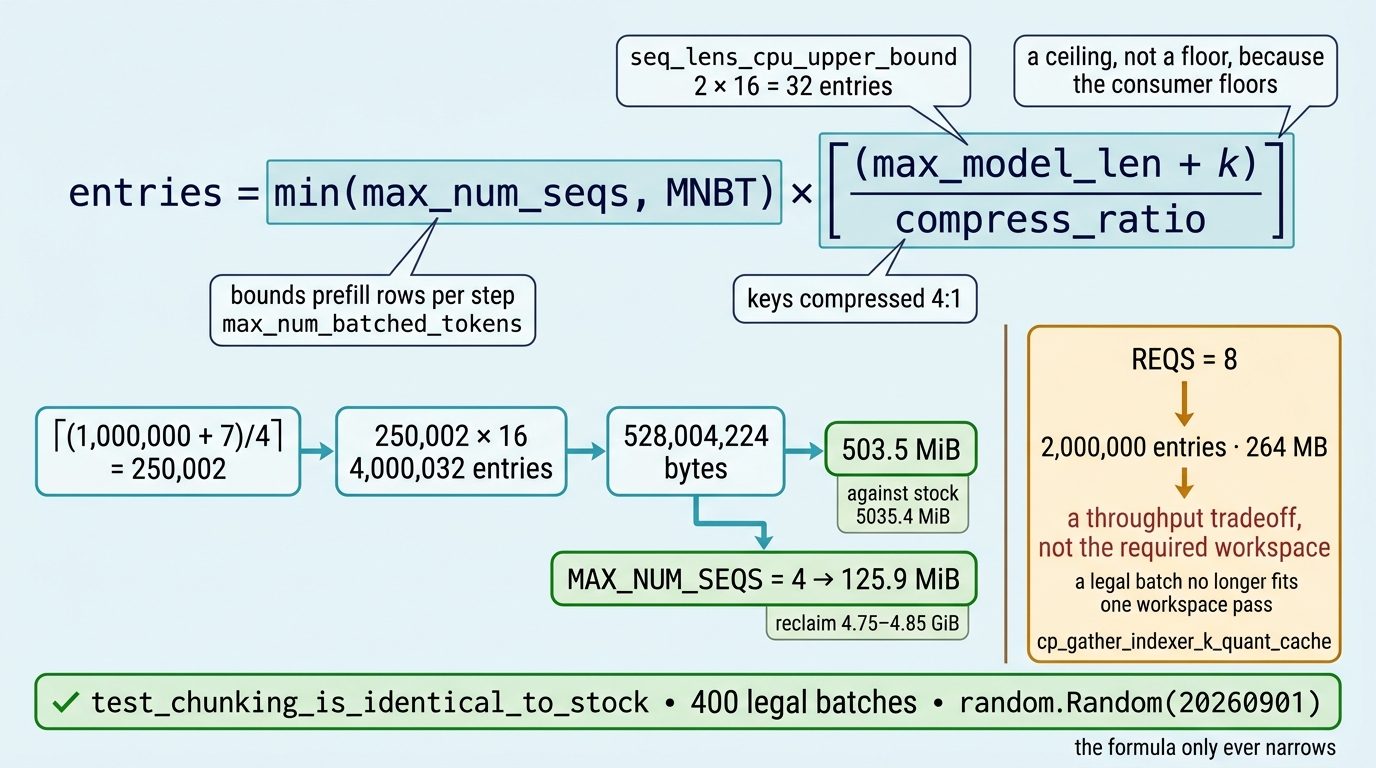
\includegraphics[width=\textwidth]{figures/ch16-legal-maximum.png}
\caption{The shipped formula, factor by factor. The $\min$ bounds how many
prefill requests one step can carry, because every prefill row costs at least
one query token of the \code{max_num_batched_tokens} budget; the $+k$ covers
the scheduler's \code{seq_lens_cpu_upper_bound}, which the drafter's seven
speculative tokens can push past \code{max_model_len}; and the division is a
ceiling rather than a floor because the consumer floors. At the live
configuration this yields 250{,}002 compressed entries per request and
4{,}000{,}032 in total --- 528{,}004{,}224 bytes, 503.5\,MiB against the stock
5035.4\,MiB, and 125.9\,MiB at the shipped \code{MAX_NUM_SEQS=4}. The first
draft's tuned \code{REQS=8} sizing was rejected as ``a throughput tradeoff,
not the required workspace'': under it a legal batch of sixteen 1M-context
thin prefills no longer fits in one workspace pass.
\code{test_chunking_is_identical_to_stock} replays 400 randomly generated
legal batches to prove the shipped sizing changes nothing, and a companion
power test proves the equivalence test can fail.}
\label{fig:proof-legalmax}
\end{figure}

\begin{hblesson}
When reclaiming a reservation, compute the legal maximum, never a tuned
estimate. A tuned number trades an invisible amount of behavior for memory and
must be re-measured on every geometry change; a legal maximum is a theorem
about the code, valid until the code changes --- at which point a fail-closed
guard should turn the invalidated assumption into a boot error instead of a
silent under-size. And pair every ``nothing changed'' equivalence test with a
power test proving the test can detect a change, or the equivalence claim is
untestable by construction.
\end{hblesson}

\subsection{An enum, because a typo must not pick a serving mode}

Activation is deliberately rigid. \envvar{GLM53_INDEXER_WORKSPACE} accepts
exactly two literal strings, \code{stock} (the default; unset means stock,
byte-for-byte the original expression) and \code{rightsize}. Everything else
--- \code{""}, \code{" rightsize "}, \code{RIGHTSIZE}, \code{1}, \code{on},
\code{right-size} --- is rejected at launch, on the grounds the launcher
comment states outright: ``a typo'd knob must not silently pick a serving
mode.''

The rule has a scar. PR~38 (hecisaza's numeric-knob
validation) landed after a \envvar{GPU_MEM_UTIL=8.7} typo took down a
healthy two-node deployment before being diagnosed: \code{./start.sh
restart} calls \code{stop} before vLLM can even parse the bad value, so the
typo killed a working serve rather than being rejected by it. Hence
validate-before-dispatch --- \code{validate_numeric_config()} now runs
before the restart is allowed to touch anything, and the byte-literal enum
here inherits the same posture.

The same accept/reject set is implemented twice, once in the bash
launcher's \code{_glm53_validate_enum} and once in the Python patch. A
test executes \emph{both} implementations over the same value list and diffs
their verdicts value-for-value, so a knob cannot change meaning across the
container boundary. Even the rejected result is clamped: the formula only ever
narrows, and a configuration whose legal maximum exceeds stock keeps stock and
logs the upstream latent risk instead of pretending to fix it.

\section{The guard that guarded the wrong case}
\label{sec:proof-guard}

A proof is only as durable as the guard that watches its assumptions, and
the guard is where this patch earned its scar: the first draft of its
fail-closed cross-check carried a conditional that read as an optimization
and was, in fact, a hole. The story is best told as it unfolded.

\begin{hbwarstory}
The right-sizing patch shipped with a fail-closed cross-check --- and the first
draft of that cross-check contained the chapter's best bug. The sizing formula
can only read \code{hf_text_config.index_kpool}; the authoritative runtime
value, \code{kv_cache_spec.compress_ratio}, resolves later, in the metadata
builder's \code{__init__}. ``Same number by construction, but construction is
not a check,'' so the patched builder compares them at init on every TP rank.
The PR~8 draft wrote the comparison as:

\begin{lstlisting}[language=Python]
# PR-8 draft -- rejected by review as a blocker
if mode == "rightsize" and self.compress_ratio > 1:
    ...cross-check...

# shipped form -- unconditional, both directions
if mode == "rightsize":
    ...raise on any index_kpool/compress_ratio mismatch...
\end{lstlisting}

The \code{compress_ratio > 1} clause looks like a harmless optimization ---
uncompressed models have nothing to cross-check. It skips exactly the one
combination that under-sizes: \code{index_kpool=4} in the config with a
runtime \code{compress_ratio} of 1. In that state the workspace is sized for
compressed pools (4{,}000{,}032 entries) while the runtime hands the splitter
raw token counts. The worst case is $16 \times 1{,}000{,}007 \approx 16$M
entries, which the regression test asserts is more than $3.9\times$ the sized
workspace: ``$\sim$4x under-sized, uncaught.'' The Codex review flagged it as
a blocker; the shipped guard raises unconditionally, in both mismatch
directions, naming \code{index_kpool}, \code{compress_ratio}, and the env var
in the error. Direction B --- config says uncompressed, runtime compresses ---
cannot under-run, but ``the two config sources disagree about the model and
rightsize must not serve on that.''
\end{hbwarstory}

The lockdown that followed is as instructive as the bug. The test suite pins
the fix three ways: \code{test_builder_ratio_mismatch_raises_both_directions}
exercises \emph{both} mismatch directions behaviorally;
\code{test_builder_guard_has_no_ratio_condition} pins the \emph{source form},
asserting the shipped guard text no longer contains the old
\code{if _glm53_workspace_mode() == "rightsize" and self.compress_ratio}
conditional --- because behavioral tests alone could pass against a merely
reordered guard; and the builder additionally raises if the allocated
workspace is ever below the legal per-step maximum, so a future resize in
either direction trips the same wire. A guard that skips its worst case is
worse than no guard, because it converts ``we don't check'' into ``we
checked.'' The review treated that as a blocker, and the tests make the
mistake unrepeatable --- \Cref{fig:proof-guardcell} shades the cell the
condition skipped.

\begin{figure}[htbp]
\centering
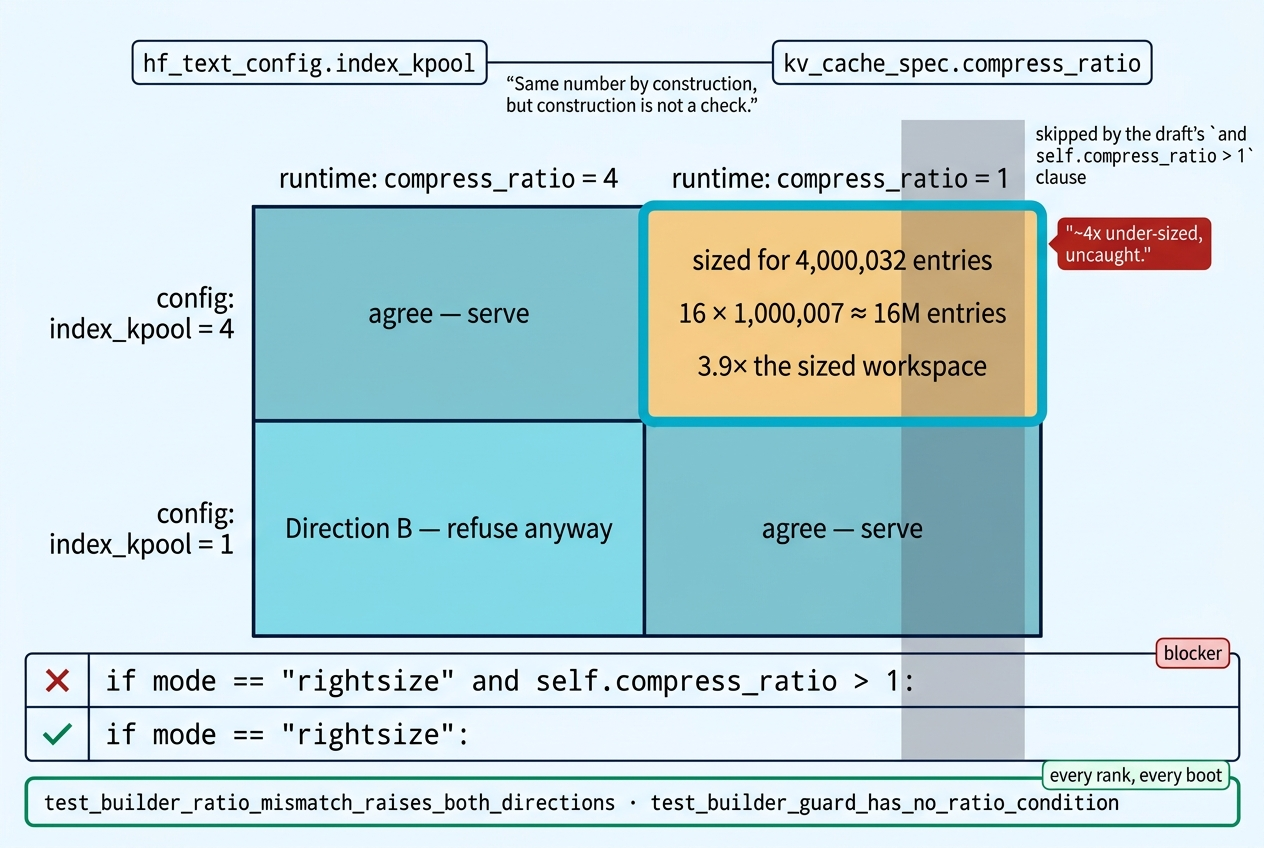
\includegraphics[width=\textwidth]{figures/ch16-guard-cell.png}
\caption{The four states of a two-source cross-check. The sizing formula can
only read \code{hf_text_config.index_kpool}, while the authoritative
\code{kv_cache_spec.compress_ratio} resolves later in the metadata builder's
\code{__init__} --- ``same number by construction, but construction is not a
check.'' The PR~8 draft guarded the comparison behind
\code{self.compress_ratio > 1}, which reads as a harmless optimisation and in
fact shades out the entire right-hand column, including the one cell that
under-sizes: config says pools, runtime hands raw token counts, and a worst
case of $16 \times 1{,}000{,}007 \approx 16$M entries meets a workspace sized
for 4{,}000{,}032 --- over $3.9\times$ under. The shipped guard raises
unconditionally in both directions, on every rank at every boot, and three
tests pin it: two behavioural, one on the source form itself, because a
behavioural test alone could pass against a merely reordered guard.}
\label{fig:proof-guardcell}
\end{figure}

\section{Smaller reclaims, same doctrine}
\label{sec:proof-smaller}

The same doctrine operates at a second scale, one order of magnitude down.
vLLM subtracts a CUDA-graph memory \emph{estimate} from the KV pool before
capture. On this kit the estimate is 2.43\,GiB, while the captured graphs,
once measured, actually consumed $-0.19$\,GiB --- at or below zero net. The
2.43\,GiB deduction was pure pessimism: roughly 2.6\,GiB of KV reserved and
never used. PR~25's
\envvar{CG_ESTIMATE=0} keeps CUDA graphs fully on and drops only the
deduction: again, not a tuning knob but the replacement of a pessimistic guess
with a measured actual, reclaiming capacity with no change to what executes.
The estimator anomaly and the workspace sit on the same ledger in
\Cref{tab:proof-reclaims}. Between them, the two dated boot receipts bracket
the pool's growth: the 2026-08-28 serve booted a 1{,}754{,}237-token KV
pool, and the 2026-09-01 validated boot (MNBT 7168, the E2 prefill kernel, and
\code{rightsize} together) reports 1{,}243{,}902 tokens at a different
geometry --- each quoted from the allocator's own startup lines rather than
derived arithmetic.

The habit of cross-checking one value from two sources, in both directions,
also outlived the guard that taught it: the shipped builder init verifies
\code{index_kpool} against \code{compress_ratio} on every rank at every boot,
unconditionally. On this recipe, an assumption a proof depends on is never
checked once at patch time --- it is re-verified at every boot, on every rank,
and a disagreement refuses to serve. Every byte reclaimed this way lands in
the KV pool; whether prompts can actually \emph{reuse} that pool is the
question the rest of the chapter turns to.

\section{The prefix cache is page-quantized}
\label{sec:proof-prefixpage}

\subsection{Only whole pages count}

The second half of the byte story begins with a fact about the KV layout from
\Cref{ch:quantized-bet}'s hybrid geometry: the sparse-MLA \code{KpoolTailManager} disables
fine-grained prefix-cache hits, so only \emph{block-aligned} tokens count, and
the alignment is the 3{,}584-token hybrid MLA page. A warm prompt reuses
exactly $\lfloor \text{tokens} / 3584 \rfloor \times 3584$ tokens --- nothing
in between. The consequences are counter-intuitive enough that the repository built
a bench around them (\Cref{fig:proof-pagehits}): a 6.8k-token conversation
reuses \emph{one} page (3{,}584 tokens, roughly 53\,\% of its prompt), while a
7.7k conversation reuses two (7{,}168 tokens, roughly 93\,\% --- ``the
upstream headline''). Two prompts a mere 900 tokens apart in length sit forty
percentage points apart in reuse, because one of them crosses a page boundary
and the other does not. The practical form of this is that prompt length buys
reuse in steps rather than in proportion: the token that completes a page is
worth 3{,}584 tokens of recomputation, and the one after it is worth nothing
until 3{,}583 more arrive.

\begin{figure}[htbp]
\centering
\adjustbox{max width=\textwidth}{%
\begin{tikzpicture}[font=\small]
  % scale: 0.9 mm per 100 tokens -> 0.9 cm per 1000 tokens
  \def\ppx#1{#1*0.09}
  % page boundary grid
  \foreach \b/\lab in {0/0, 35.84/3584, 71.68/7168, 107.52/10752} {
    \draw[hbSteel!50,dashed] (\ppx{\b},0.4) -- (\ppx{\b},-3.3);
    \node[hblabel,anchor=south] at (\ppx{\b},0.45) {\lab};
  }
  \node[hbtitle,anchor=south west] at (\ppx{0},1.0)
    {3584-token page boundaries (block-aligned hits only)};
  % prompt A: 6.8k
  \fill[hbGreen!35] (0,-0.5) rectangle (\ppx{35.84},-1.15);
  \fill[hbGray]    (\ppx{35.84},-0.5) rectangle (\ppx{68},-1.15);
  \draw[hbSteel,thick] (0,-0.5) rectangle (\ppx{68},-1.15);
  \node[hblabel,anchor=west] at (\ppx{68}+0.15,-0.82)
    {6.8k prompt: 1 full page = 3584 hit tokens ($\approx$53\,\%)};
  % prompt B: 7.7k
  \fill[hbGreen!35] (0,-1.75) rectangle (\ppx{71.68},-2.4);
  \fill[hbGray]    (\ppx{71.68},-1.75) rectangle (\ppx{77},-2.4);
  \draw[hbSteel,thick] (0,-1.75) rectangle (\ppx{77},-2.4);
  \node[hblabel,anchor=west] at (\ppx{77}+0.15,-2.07)
    {7.7k prompt: 2 full pages = 7168 hit tokens ($\approx$93\,\%)};
  % legend
  \fill[hbGreen!35] (0,-3.05) rectangle (0.4,-2.75);
  \node[hblabel,anchor=west] at (0.5,-2.9) {reused (cache hit)};
  \fill[hbGray] (3.6,-3.05) rectangle (4.0,-2.75);
  \node[hblabel,anchor=west] at (4.1,-2.9) {recomputed (below the next boundary)};
\end{tikzpicture}%
}
\caption{Page-quantized prefix reuse. The hybrid KV layout counts hits only in
whole 3584-token MLA pages: a 6.8k-token warm prompt reuses one page
($\approx$53\,\% hit ratio) while a 7.7k prompt reuses two ($\approx$93\,\%).
\repofile{tests/bench_prefix_cache.py} scores measured hits against this page
model as \code{hit_efficiency} and defaults to 8{,}400 prompt tokens so its
warm turn crosses the second boundary.}
\label{fig:proof-pagehits}
\end{figure}

\subsection{A bench that scores itself against the model}

\repofile{tests/bench_prefix_cache.py} makes the page model executable. Each
run stages a cold turn (system prompt plus a long unique document) and a warm
follow-up that resends the identical history, reading
\code{vllm:prefix_cache_hits} and \code{queries} counter deltas around each
turn. Its headline metric is not the raw hit ratio but
\code{hit_efficiency}: measured hit tokens divided by the full-page
expectation $\lfloor \text{tokens}/3584 \rfloor \times 3584$. A value of 1.0
means the page model is being respected; the tool warns when the median falls
below 0.9, meaning either the warm prompt fails to cross a full page boundary
or reuse is partial. The default \code{--prompt-tokens 8400} is chosen to land
about 8.1k measured tokens --- safely across the second boundary --- so an
out-of-the-box run exercises a two-page hit rather than teetering on one
(\Cref{tab:proof-hits}).

\begin{center}
\small
\captionof{table}{The 3584-token page model against measured reuse. Model
rows follow $\lfloor\text{tokens}/3584\rfloor \times 3584$; the measured row
is the 2026-08-29 cold-prefill ladder's APC follow-up receipt.}
\label{tab:proof-hits}
\begin{tabular}{@{}rrrr>{\raggedright\arraybackslash}p{4.0cm}@{}}
\toprule
Prompt tokens & Full pages & Hit tokens & Hit ratio & Note \\
\midrule
6{,}800 & 1 & 3{,}584 & $\approx$53\,\% & below the second boundary \\
7{,}700 & 2 & 7{,}168 & $\approx$93\,\% & ``the upstream headline'' \\
8{,}004 & 2 & 7{,}168 & 89.6\,\% & measured: warm TTFT 1.30\,s after a
  10.36\,s cold (2026-08-29) \\
14{,}336 & 4 & 14{,}336 & 100\,\% & exactly four pages \\
\bottomrule
\end{tabular}
\end{center}

\subsection{Cold means salted: the 5$\times$ TTFT swing}

The page model also explains why this repository's cold benchmarks are paranoid.
This vLLM build exposes no cache-reset endpoint, so a ``cold'' measurement is
only cold if no previous session cached its pages. On 2026-08-29 two bench
sessions disagreed by $5\times$ on cold TTFT; the reruns had reused chat
content, and the supposedly cold turn dropped from 10.3\,s to 1.9\,s on
recycled pages. The fix is baked into the harnesses rather than into
operator discipline. \repofile{tests/bench_prefix_cache.py} injects a
per-invocation session salt into every checksum string of its filler
document, and the cold-prefill ladder
(\repofile{tests/_run_cold_prefill.py}, protocol in
\repofile{docs/cold-prefill.md}) puts a unique UUID-plus-hex-pad salt
\emph{first} in every user message so the prefix cache cannot cheat. Both
instrument their own cold turns with per-request metric deltas
(\code{prefix_cache_hits_total},
\code{prompt_tokens_by_source_total\{source="local_compute"\}}), so a cold
rung that actually hit cache is self-incriminating --- the same
distrust-your-own-benchmark reflex \Cref{ch:measurement} institutionalized, now applied
to a cache that never forgets.

\needspace{5\baselineskip}
\section{Prompt bytes as a performance interface}
\label{sec:proof-pr63}

\subsection{The PR~63 story: a one-line guard, a full re-prefill}

The page model has a corollary the lab learned the expensive way: the bytes
at the very head of a prompt hold every page behind them hostage.

\begin{hbwarstory}
vLLM chains prefix-cache block hashes forward from token 0, and on this serve
only whole 3{,}584-token pages count. So any divergence near the head of the
prompt invalidates \emph{everything} behind it. The kit's chat template
rendered a \code{<|system|>Reasoning Effort: X} header at the very start of
the prompt --- but gated it on \code{thinking_enabled}. Toggle thinking off,
and the header disappears: the thinking-on and thinking-off renderings of the
same conversation diverge at roughly token~2. With tools present --- and agent
traffic always carries tools --- the two prompts shared 22 characters out of
855. Every thinking toggle therefore re-prefilled the world. Measured on a
21{,}642-token prompt, toggling reasoning effort high$\to$none cost a full
cold prefill, 26.54\,s; after the fix, the same toggle completed in
0.42\,s warm. The fix (PR~63, contributed by sovereignbrah, commit
\code{4753ac2}: ``emit Reasoning Effort unconditionally to keep the prefix
cache'') is one line of template logic --- and it also restores the upstream
zai-org template's behavior, which the guard had quietly forked.
\end{hbwarstory}

The repaired template treats prompt-prefix stability as a tested contract, not
a hope (\Cref{fig:proof-divergence}). \code{<|system|>Reasoning Effort: Max}
is rendered at position 0 of every prompt, in \emph{both} thinking modes.
Thinking is disabled by pre-closing the block, so the generation prompt ends
\code{<|assistant|><think>} when thinking is on and
\code{<|assistant|><think></think>} when it is off. That makes the
thinking-off prompt a \emph{strict string extension} of the thinking-on
prompt, with suffix exactly \code{</think>}.
\repofile{tests/test_chat_template.py} asserts precisely that --- both without
tools and, critically, with tools present, ``because agent traffic always
carries tools; the tools block renders after the reasoning-effort line, so
this is the case that actually regressed.''

The general form is worth extracting: when two renderings of the same
conversation must both hit a page-granular cache, make one a strict extension
of the other rather than a variant of it. Divergence in the tail costs one
page; divergence in the head costs every page behind it.

A further pin holds the effort levels themselves to a shared prefix up to the length of
\code{[gMASK]<sop><|system|>Reasoning Effort: }, so switching Max to Low
diverges as late as the token stream allows. Two pre-existing tests had
\emph{encoded the divergence} as expected behavior; PR~63 rewrote them ---
a reminder that a test suite can canonize a bug as faithfully as it canonizes
a fix.

\begin{figure}[htbp]
\centering
\adjustbox{max width=\textwidth}{%
\begin{tikzpicture}[font=\small]
  % BEFORE panel
  \node[hbtitle,anchor=west] at (0,1.1) {Before PR~63: header gated on thinking};
  % thinking on row
  \node[hblabel,anchor=east] at (-0.15,0.3) {thinking on};
  \fill[hbGreen!35] (0,0) rectangle (0.9,0.6);
  \fill[hbBlue!20] (0.9,0) rectangle (5.6,0.6);
  \fill[hbGray] (5.6,0) rectangle (10.6,0.6);
  \draw[hbSteel,thick] (0,0) rectangle (10.6,0.6);
  \node[font=\scriptsize] at (3.25,0.3) {\texttt{<|system|>Reasoning Effort: Max}};
  \node[font=\scriptsize] at (8.1,0.3) {tools + history (855 chars)};
  % thinking off row
  \node[hblabel,anchor=east] at (-0.15,-0.75) {thinking off};
  \fill[hbGreen!35] (0,-1.05) rectangle (0.9,-0.45);
  \fill[hbAccent!25] (0.9,-1.05) rectangle (10.6,-0.45);
  \draw[hbSteel,thick] (0,-1.05) rectangle (10.6,-0.45);
  \node[font=\scriptsize] at (5.75,-0.75) {header dropped $\rightarrow$ diverges at token 2 (22/855 shared chars)};
  \draw[hbfail] (0.9,-1.3) -- (10.6,-1.3)
    node[hblabel,midway,anchor=north,yshift=-0.5mm]
    {every thinking toggle = full re-prefill: 26.54\,s on a 21{,}642-token prompt};
  % AFTER panel
  \node[hbtitle,anchor=west] at (0,-2.6) {After PR~63: header unconditional, off = strict extension};
  \node[hblabel,anchor=east] at (-0.15,-3.4) {thinking on};
  \fill[hbGreen!35] (0,-3.7) rectangle (9.2,-3.1);
  \draw[hbSteel,thick] (0,-3.7) rectangle (9.2,-3.1);
  \node[font=\scriptsize] at (4.6,-3.4)
    {\texttt{Reasoning Effort: Max} at position 0 + tools + history + \texttt{<think>}};
  \node[hblabel,anchor=east] at (-0.15,-4.45) {thinking off};
  \fill[hbGreen!35] (0,-4.75) rectangle (9.2,-4.15);
  \fill[hbAmber!35] (9.2,-4.75) rectangle (10.6,-4.15);
  \draw[hbSteel,thick] (0,-4.75) rectangle (10.6,-4.15);
  \node[font=\scriptsize] at (4.6,-4.45) {identical prefix, byte for byte};
  \node[font=\scriptsize] at (9.9,-4.45) {\texttt{</think>}};
  \draw[hbok] (0,-5.0) -- (9.2,-5.0)
    node[hblabel,midway,anchor=north,yshift=-0.5mm]
    {shared prefix survives the toggle: 0.42\,s warm};
\end{tikzpicture}%
}
\caption{The token-2 divergence and its repair. Before PR~63 the
reasoning-effort header was gated on \code{thinking_enabled}, so thinking-on
and thinking-off prompts shared only 22 of 855 characters with tools present
and every toggle re-prefilled from scratch (26.54\,s at 21{,}642 tokens).
After the fix the header renders unconditionally at position 0 and the
thinking-off prompt is a strict extension of the thinking-on prompt with
suffix exactly \code{</think>} --- the toggle became a 0.42\,s warm hit.}
\label{fig:proof-divergence}
\end{figure}

\subsection{The client side of the interface}

If prompt bytes are an interface, clients are counterparties, and the repository
ships its reference client configuration under \repofile{examples/pi/} --- a
throughput-honest budget for pointing a coding agent at this serve. The Pi
configs hard-wire \code{chat_template_kwargs} with \code{enable_thinking}
false, so every agent request rides the exact thinking-off template shape the
prefix-stability tests pin. They cap the client's \code{contextWindow} at
500{,}000 tokens --- deliberately half the server's 1M
\code{max_model_len} --- and they bound agent concurrency to
\code{maxConcurrent: 2} subagents (one foreground), matched to the recipe's
small \code{MAX_NUM_SEQS}. Two Sparks serving roughly 37 \tokspersec{} per
stream under four-way concurrency cannot feed an unbounded agent swarm, and
the configuration says so in numbers rather than in a warning nobody reads.

\section{Two starvation and corruption guards in the same spirit}
\label{sec:proof-guards}

Two more overlay patches close the chapter, and they bracket the two costs
of sharing one pool of bytes among heterogeneous consumers. The scheduler
shares a token budget and must sometimes refuse to (starvation); the KV
groups share a block pool and must be prevented from writing across each
other (corruption). Each fix is a small, provable intervention at a
precisely identified boundary, shipped with a test that encodes the
incident.

\subsection{The decode floor: refuse to share the step}

Issue \ghissue{6} in the GLM kit's tracker records the symptom: mixed decode
was roughly $11\times$ slower than solo decode. The engine step budget
(1{,}024 tokens at the time) is shared; a decode lane needs about 8 tokens
(one bonus plus the drafter's $k{=}7$), and the leftover $\sim$1{,}016 went to
a peer's sparse-MLA cold-prefill chunk costing $\sim$1.5\,s per step. Decode
still ran --- at $\sim$5 \tokspersec{} instead of $\sim$50. The instinctive
fix, capping mixed prefill at 128 tokens, was tried and was \emph{not
enough}: the sparse indexer carries a large per-step fixed cost, and mixed
decode still crawled at $\sim$10 \tokspersec{} on an 80k-token KV. So
\repofile{overlay/patch_scheduler_decode_floor.py} skips mixed prefill
entirely: while any peer is decoding, waiting prefills are deferred to the
next step and running-queue prefills are capped, resuming at full chunk size
the moment no one decodes. (\envvar{GLM53_MIXED_PREFILL_CHUNK=skip};
\code{N>0} is available as a cap for operators who want to mix anyway.) The live
regression test, \repofile{tests/test_mixed_prefill_decode.py}, decodes one
lane solo, then again while a second lane cold-prefills, and fails at a solo-to-mixed ratio above $5\times$ --- the comment is explicit that $11\times$
was the disease and $\sim$3$\times$ is tolerable overlap.

The asymmetry is what generalizes past this scheduler: when one lane's unit
of work costs about eight tokens of the step budget and another's costs a
thousand, splitting the budget fairly does not split the latency fairly, and
the cheap remedy is to refuse the mix while anyone is decoding, as
\Cref{fig:proof-mixeddecode} lays out.

\begin{figure}[htbp]
\centering
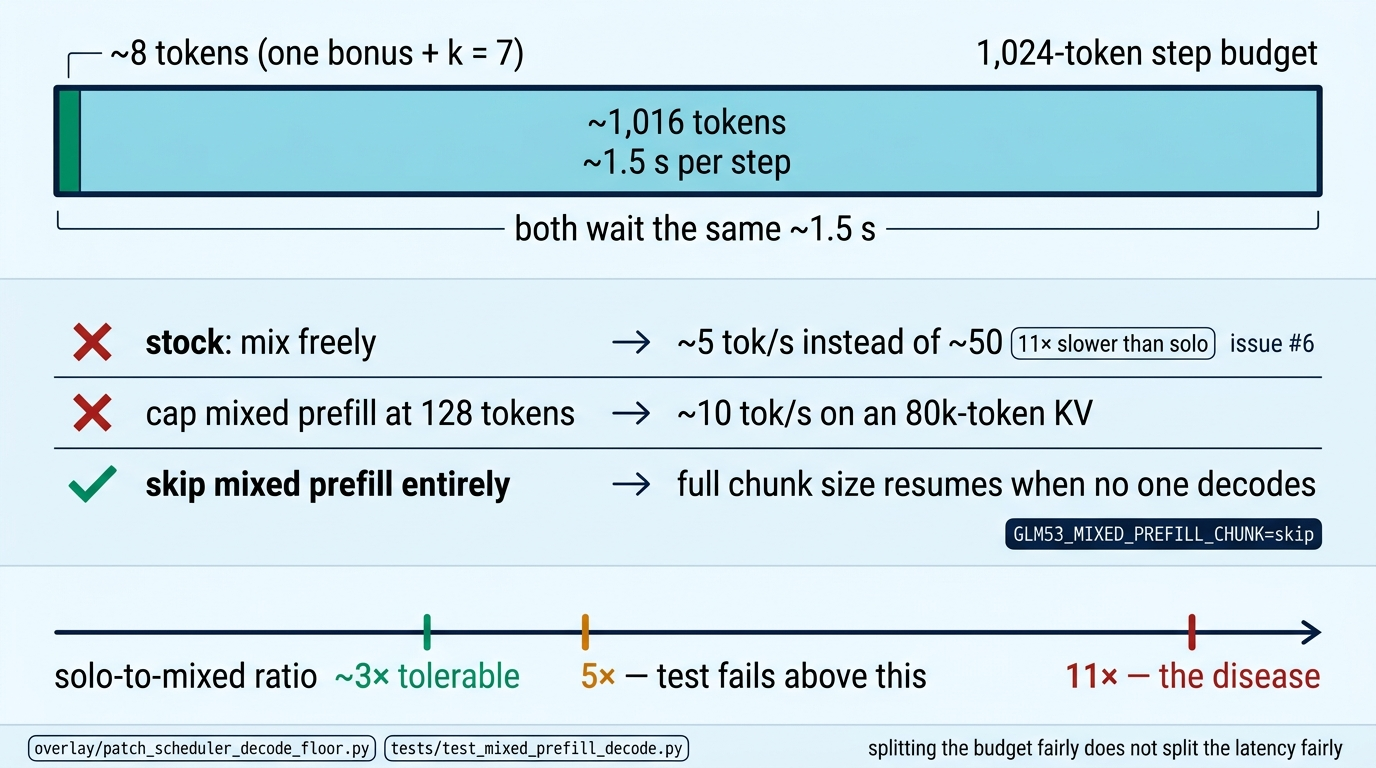
\includegraphics[width=\textwidth]{figures/ch16-mixed-decode.png}
\caption{Why a fair split of the step budget is not a fair split of latency. A
decode lane needs about 8 tokens of the 1{,}024-token engine step --- one
bonus plus the drafter's seven --- while the leftover $\sim$1{,}016 admit a
peer's sparse-MLA cold-prefill chunk costing about 1.5\,s per step, and both
lanes then wait it out: decode ran at $\sim$5 \tokspersec{} instead of
$\sim$50, roughly $11\times$ slower than solo. The instinctive remedy of
capping mixed prefill at 128 tokens was tried and was not enough --- the
sparse indexer carries a large per-step fixed cost, and mixed decode still
crawled at $\sim$10 \tokspersec{} on an 80k-token KV --- so the shipped policy
skips mixed prefill entirely while any peer is decoding, resuming full chunk
size the moment no one does. The live regression test fails above a $5\times$
solo-to-mixed ratio; $\sim$3$\times$ is tolerable overlap.}
\label{fig:proof-mixeddecode}
\end{figure}

\subsection{The one-line clamp: corruption that lands elsewhere}

The kpool tail is a one-block circular scratch cache: block size equals
\code{index_kpool} (4), and its block-table row holds a \emph{single} entry.
vLLM's generic paged slot-mapping Triton kernel computes
\code{block_indices = pos // block_size} and indexes the row with a mask that
guards only token validity --- nothing bounds the index against the row's
width. For the tail group, every token at \code{pos >= block_size} reads past
the one entry, and the kpool seed and update kernels then write through
whatever garbage block id came back. Generations of roughly 2{,}000 tokens
hit it reliably. The failure is insidious in exactly the way silent
corruption always is: a finished request is not proof the writes were
in-bounds, because most overruns land inside the shared pool and corrupt
\emph{another layer's} indexer state.

The fix in
\repofile{overlay/patch_kpool_tail_slotmap.py} is one Triton line:
\code{tl.minimum(block_indices, block_table_stride - 1)}. For the
tail's stride-1 row it restores the circular addressing the seed kernel
already documents, and it is provably an identity for every other KV group,
since no other group legitimately needs more blocks than its row holds. The
mechanism was credited to a sibling community recipe's write-up
(\repofile{docs/KPOOL_TAIL_BUG.md} in vcruz305's GLM Spark recipe). The
host test pins the arithmetic: with row \code{[17]} and block size 4,
positions 0--63 must wrap onto the same four slots, and the \emph{unclamped}
mapping must raise an index error at position 4 --- proof the patch is load-bearing, not decorative.

\begin{hbnote}
Both fixes are small because the analysis was exact; both carry tests that
reproduce the incident rather than merely asserting the patch applied.
\end{hbnote}

\FloatBarrier

Two things in this system have quietly changed category. A reservation is
no longer a number somebody once chose --- it is a claim about the largest
request the scheduler is permitted to construct, and where nobody has
re-derived that claim, the distance between it and the truth sits locked in
the process for the life of the serve. And a prompt is no longer text: on a
cache that counts only whole 3{,}584-token pages, the first twenty bytes of
a rendering decide whether the twenty thousand behind them are free or cost
26.54 seconds. Bytes are held by allocations and by strings alike, and both
classes yield to the same instrument --- a bound, plus a guard that fails
closed the moment the bound's assumptions drift.

\section*{Takeaways}

\begin{itemize}
  \item Reconcile before you reclaim, then size by legal maximum rather
    than tuned estimate: the 5036.40\,MB receipt was reproduced to the byte
    from the sizing formula before anyone patched it
    (\Cref{sec:proof-workspace}), and the shipped bound's chunk list is
    provably identical to stock over 400 random legal batches where the
    rejected REQS${=}8$ tuning would have silently split legal prefills ---
    4.75--4.85\,GiB returned to the KV pool at the shipped
    \code{MAX_NUM_SEQS=4}.
  \item A proof is only as durable as the guard around it. Guards must
    cover their worst case --- the \code{compress_ratio > 1} clause skipped
    exactly the combination that under-sizes --- and every equivalence test
    needs a power test proving it can fail, or ``nothing changed'' is
    unfalsifiable.
  \item A page-granular prefix cache makes prompt bytes an interface: one
    conditional header cost every thinking toggle a full re-prefill ---
    26.54\,s on a 21{,}642-token prompt --- until PR~63 made thinking-off a
    strict extension of thinking-on (\Cref{sec:proof-pr63}). Test the
    template shape your traffic actually has: that regression only
    manifested with tools present.
  \item Cold benchmarks must prove their own coldness: on a serve with no
    cache-reset endpoint, where recycled pages once swung cold TTFT by
    5$\times$, prompt salting plus per-request hit-counter deltas make a
    cache-hit cold rung self-incriminating.
  \item Small exact interventions beat broad tuning: a skip-mixed-prefill
    policy against the $11\times$ decode collapse and a one-line
    \code{tl.minimum} clamp against cross-layer KV corruption, each shipped
    with a test that replays the incident.
\end{itemize}

\chaptertransition{Every discipline in this chapter is the same move made
at a different scale: bound the claim, then refuse to serve where the bound
stops. The last chapter of the GLM story runs that move against the two
things a serving recipe is least able to prove --- the weights themselves,
and hardware the lab does not own --- and closes on the open repository
where community pull requests, human and AI co-authored alike, arrive
carrying their own receipts. It opens with a published refusal direction
that is mathematically immaculate and, measured against stock \code{o_proj},
indistinguishable from a random unit vector: which leaves the question of
how you edit a 320B-class model's behavior at load time once the elegant
method has failed its own measurement.}
